\begin{frame}{\makebox[0pt][l]{
\includegraphics[scale=0.3]{Logotip.png}}\hspace{4cm}\textbf{\textcolor{blue}{М}\textcolor{gray}{ера количества информации по Шеннону}}}
    
    \begin{wrapfigure}{tr}{0.3\textwidth}
        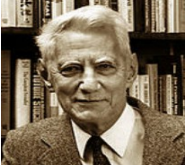
\includegraphics[width = 0.9\linewidth]{Slide18.png}
        \caption*{Клод Шеннон\\(1916--2001)}
    \end{wrapfigure}
    
    \fontsize{9pt}{11pt}\selectfont
    \setlength{\parindent}{3ex}
    \noindentМера Хартли подходит лишь для систем с равновероятными состояниями.Если состояния системы S не равновероятны, используют меру Шеннона:
    \begin{equation*}
        i(S) = -\sum_{i = 1}^{N} p_i \cdot \log_2 p_i,
    \end{equation*}
    \noindentгде $N$ – число состояний системы,\\
    \noindent$p_i$ – вероятность того, что система S находится в\\
    \quadсостоянии $i$ (сумма всех $p_i$ равна 1).
    
    \medskip
    \fontsize{11pt}{13pt}\selectfont\textcolor{Green}{Формула Хартли является частным случаем формулы Шеннона!}
    
    \smallskip
    \fontsize{9pt}{11pt}\selectfont\noindent\textbf{Пример 1.} Количество информации в акте подбрасывания обычной монеты по формуле Хартли равно $\log_2 2$ = 1 бит. По формуле Шеннона получим то же: $i_{s1}$ = -0,5*$\log_2 0,5$ - 0,5*$\log_2 0,5$ = 1 бит.\\
    \noindent\textbf{Пример 2.} При подбрасывании монеты со смещённым центром тяжести количество непредсказуемости становится меньше: $i_{s2}$ = -0,75*$log_2 0,75$ - 0,25*$log_2 0,25$ $\approx$ 0,8 бит. 

\end{frame}